

\documentclass[xcolor=table]{beamer}
\usetheme{default}
\definecolor{darkscarlet}{rgb}{0.34, 0.01, 0.1}
\usecolortheme{default}
\usecolortheme[named=darkscarlet]{structure}
\setbeamercolor{title}{bg=white, fg=darkscarlet}
\definecolor{cerise}{rgb}{0.87, 0.19, 0.39}
\hypersetup{colorlinks=TRUE,linkcolor=cerise,urlcolor=cerise, citecolor=cerise}

% nummering

\setbeamertemplate{caption}[numbered]

% taal

\usepackage[english]{babel}

% tekens

\usepackage{fontspec}
\usefonttheme{serif}
\setmainfont[BoldFont=brillb.ttf, ItalicFont=brilli.ttf, BoldItalicFont=brillbi.ttf]{brill.ttf}

% tekst doorstrepen, kennelijk heb je daar een apart pakket voor nodig

\usepackage[normalem]{ulem}

% plaatjes

\usepackage{graphicx}

% tabellen

\usepackage{multirow}

% voorbeelden

\usepackage{philex}

% glossen

\usepackage{leipzig}

\newleipzig{hab}{hab}{habitual}
\newleipzig{ad}{ad}{ad}
\newleipzig{el}{el}{elative}
\newleipzig{aor}{aor}{aorist}
\newleipzig{rfl}{rfl}{reflexive}
\newleipzig{emph}{emph}{emphatic particle}
\newleipzig{pf}{pf}{perfect}
\newleipzig{lat}{lat}{lative}
\newleipzig{sup}{sup}{super}
\newleipzig{atr}{atr}{attributivizer}
\newleipzig{add}{add}{additive}
\newleipzig{in}{in}{in}
\newleipzig{rep}{rep}{reportative}
\newleipzig{msd}{msd}{masdar}
\newleipzig{aff}{aff}{affective}
\newleipzig{indef}{indef}{indefinite}
\newleipzig{trans}{trans}{translative}
\newleipzig{an}{an}{animate}
\newleipzig{inan}{inan}{inanimate}
\newleipzig{th}{th}{thematic element}
\newleipzig{ord}{ord}{ordinal numeral}
\newleipzig{temp}{temp}{temporal converb}
\makeglossaries

% bibliography

\usepackage[backend=biber,babel=other,
        bibstyle=biblatex-sp-unified,
        citestyle=sp-authoryear-comp,
        doi=false,
        maxcitenames=3,
        maxbibnames=99]{biblatex}
\addbibresource{bibliography.bib}


% custom footline

\setbeamerfont{footline}{size=\fontsize{20}{20}\selectfont}

\newcommand{\Ffootline}{\footnotesize
\insertsection
\hfill
\href{https://github.com/sverhees/2019_Animacy origin}{github/sverhees/2019\_Animacy origin}
\hfill
\insertframenumber/\inserttotalframenumber} 

% custom footline deel 2

\setbeamertemplate{footline}{%
\usebeamerfont{structure}
\begin{beamercolorbox}[wd=\paperwidth,ht=2.25ex,dp=1ex]{title in head/foot}%
\Tiny\hspace*{4mm} \Ffootline \hspace{4mm}
\end{beamercolorbox}}

% navigatiesymbolen uitzetten

\beamertemplatenavigationsymbolsempty
 
 
% titelpagina 

\title{Towards a tentative origin of animacy markers in Botlikh}
\author{Samira Verhees and Chiara Naccarato \\
Linguistic Convergence Laboratory at NRU HSE Moscow}
\date{Caucasian Languages: Typology and Diachrony \\
23--24.10.2019 --- Institute of Linguistics RAS, Moscow}


% links

\usepackage{hyperref}

%\newcommand\pro{\item[$+$]}
%\newcommand\con{\item[$-$]} 
\begin{document}

\begin{frame}
\titlepage
\end{frame}

\begin{frame}{Botlikh}
\begin{itemize}
    \item Botlikh > Andic group > East Caucasian language family
    \item Unwritten, 3 villages in Daghestan, \textasciitilde{}5000-8000 speakers
    \item One full reference grammar in Georgian 
    \citep{gudava1962}
    \item Two dictionaries:
    \citep{saidovaabusov2012} and \citep{alekseev2019}
\end{itemize} 
\pause
\vfill
\begin{block}{Two gender systems}
1. Noun class (inherited)\\
2. Animacy markers (innovation)
\end{block}
\end{frame}

\section{Introduction}
\begin{frame}{Gender systems}
\begin{center}
``Grammatical gender systems generally
presuppose rather long evolutionary chains and are in this sense among the more
clearly mature elements of language.'' \citep[112]{dahl2004}
\pause
\vfill
`` [...] it appears that the half-life of a well-established gender distinction must be \textbf{several millennia}.'' \citep[200]{dahl2004}
\end{center}
\end{frame}

\begin{frame}{Gender systems and their origins}

In case a source is known, it is nominal, cf. \citep{corbett1991, audring2016}.

\vfill

\begin{figure}[h]
\centering
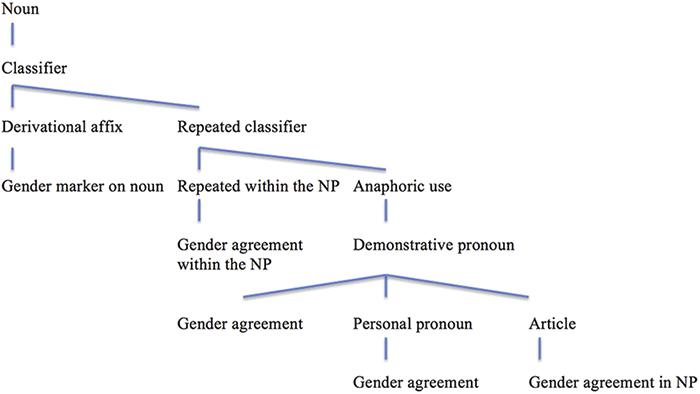
\includegraphics[scale=0.35]{images/gender.jpg}
\end{figure}

\tiny{Image from \citep{audring2016}}

\end{frame}

\begin{frame}{Aim}

\begin{center}
  \color{darkscarlet}\textbf{Aim of this talk} \\ \color{black}Discuss a gender agreement system that seems to be a unique innovation of Botlikh, and argue that the markers involved are plausibly of verbal origin.
\end{center}
    
\end{frame}


\section{Animacy}
\begin{frame}{Animacy markers}

Pairwise distribution of \textit{ɬ} and \textit{χ}. \\ 
Suggests a distinct lexical source for each ``series''.

\begin{table}[H]
\caption{Animacy markers in Botlikh}
\begin{center}
\label{tab:animparad}
\begin{tabular}{llll}
\multicolumn{2}{c}{Target}                 & \multicolumn{1}{c}{Animate} & \multicolumn{1}{c}{Inanimate} \\ \hline
\multicolumn{2}{l}{Negative copula}        & ɬi-č'i                      & χu-č'i                        \\
\multicolumn{2}{l}{Interrogative particle} &                             &                               \\
                  & Polar                  & =ɬi.ma                      & =χu.ma                        \\
                  & Content                & =ɬi.la                      & =χu.la                        \\
\multicolumn{2}{l}{Attributive clitic}     & -ɬa-cm*                     & -χo-cm                        \\
\multicolumn{2}{l}{Participle}             &                             &                               \\
                  & Present                & -ɬa-cm*                     & -χa-cm                        \\
                  & Future                 & -ɬa-cm*                     & -χa-cm                        \\
\multicolumn{2}{l}{Ordinal numeral}        & -ɬa-cm*                     & -χa-cm                       
\end{tabular}
\end{center}
\end{table}
\begin{center}
\tiny{*a variant \textit{ɬo-} appears in the environment of the masculine noun class suffix \textit{-w}.}
\end{center}
\end{frame}

\begin{frame}{Animacy agreement}

\lb{}{\gll k'eji-\textbf{ɬa-j} ješi\\
two-{\An}.{\Ord}-{\F} girl\\
\trans `the second girl (= daughter)'}

\lb{}{\gll k'eji-\textbf{ɬa-b} zini\\
two-{\An}.{\Ord}-{\N} cow\\
\trans `the second cow'}

\lb{}{\gll k'eji\textbf{-χo-b} ziw\\
two-{\Inan}.{\Ord}-{\N} day\\
\trans `the second day'}
    
\end{frame}


\begin{frame}{Animacy agreement}

\begin{table}[]
\caption{Agreement patterns}
\label{tab:anagr}
\begin{center}
\begin{tabular}{llll}
\multicolumn{2}{l}{Target}                 & Controller   & Obligatoriness \\ \hline
\multicolumn{2}{l}{Negative copula}        & ? Abs          & \textit{gu-č’i}         \\
\multicolumn{2}{l}{Interrogative particle} &              &                \\
                  & Polar                  & ? Abs          & =\textit{ma}            \\
                  & Content                & ? Abs          & =\textit{la}            \\
\multicolumn{2}{l}{Attributive clitic}     & Head / ? Abs & ?              \\
\multicolumn{2}{l}{Participle}             &              &                \\
                  & Present                & Head / ? Abs & ?              \\
                  & Future                 & Head / ? Abs & ?              \\
\multicolumn{2}{l}{Ordinal numeral}        & Head / ? Abs & yes           
\end{tabular}
\end{center}
\end{table}
    
\end{frame}

\begin{frame}{Verbal origin?}
\begin{itemize}
   \item[{$+$}] The negative copulas look like a negated verb form, consisting of a root morpheme and a regular negation (though without a derivational base). It seems the animacy markers occupy the position of the lexical root:
   \begin{itemize}
       \item Cf. \textit{χ-e-wč'i} [take-\textsc{hab-neg}] `does not take' and\\ \textit{χu-č'i} [\textsc{inan.cop-neg}] `is not' % side-note: canonical gender according to Corbett should not appear in the form of roots, only as an affix or clitic
   \end{itemize}
   \pause
    \item[{$-$}] The negative copulas look similar to the interrogative particles (they use the same allomorphs for animacy agreement (\textit{ɬi} and \textit{χu}, which are followed by a suffix), yet the latter cannot form predicates, and co-occur with the copula:

\lb{}{\gll hu-ɬːi ila-ima č'ago \textbf{ida=ɬi.ma?}\\
{\Dem}-{\Gen} parents alive {\Cop}={\An}.{\Q}\\
\trans `\textbf{Are} her parents alive?'}
\end{itemize}
\end{frame}

\begin{frame}{Verbal origin?}
\begin{itemize}
   \item[{$+$}] The negative forms of the non-past participles look similar to the negative past participle forms of full verbs:
   \end{itemize} % The formant i usually appears after the stem to derive inflection / negation etc. (see present participle and negative past participle). In the negated present participle, the -i formant is repeated after -χ 
   
\begin{table}[h]
\caption{Affirmative and negative participles}
\label{tab:negptcp}
\begin{tabular}{l|lllllll}
\cline{2-8}
        & \multicolumn{7}{c|}{Affirmative}                                                                                                              \\ \hline
Past    & \textit{ih} & \textit{}   & \textit{}            & \textit{}            & \textit{}             & \textit{-a}          & \textit{-b}          \\
        & make        &             &                      &                      &                       & -\textsc{pst.ptcp}            & -\textsc{n}                   \\ \hline
Present & \textit{ih} & \textit{-i} & \textit{-χ}          & \textit{}            & \textit{}             & \textit{-a}          & \textit{-b}          \\
        & make        & -\textsc{is}         & -\textsc{inan.prs}            &                      &                       & -\textsc{ptcp}                & -\textsc{n}                   \\ \cline{2-8} 
        & \multicolumn{7}{c|}{Negative}                                                                                                                 \\ \hline
Past    & \textit{ih} & \textit{}   & \textit{}            & \textit{\textbf{-i}} & \textit{\textbf{-č'}} & \textit{\textbf{-a}} & \textit{\textbf{-b}} \\
        & make        &             &                      & -\textsc{is}                  & -\textsc{neg}                  & -\textsc{pst.ptcp}            & -\textsc{n}                   \\ \hline
Present & \textit{ih} & \textit{-i} & \textit{\textbf{-χ}} & \textit{\textbf{-i}} & \textit{\textbf{-č'}} & \textit{\textbf{-a}} & \textit{\textbf{-b}} \\
        & make        & -\textsc{is}         & -\textsc{inan.prs}            & -\textsc{is?}                 & -\textsc{neg}                  & -\textsc{ptcp}                & -\textsc{n}                  
\end{tabular}
\end{table}
\end{frame}

\begin{frame}{Verbal origin?}

\begin{itemize}
   \item[{$+$}] The markers show up on verbal forms (negative auxiliaries, participles) or forms that seem to derive from verbal forms diachronically (attributives, ordinals < participles) (A possible exception are the interrogative particles.)
    \pause
    \item[{$-$}] No straightforward eligible candidates for lexical sources
   \end{itemize}
\end{frame}

\begin{frame}{Other Andic languages}

\begin{center}
Look for possible cognates \textit{and} a similar pairwise distribution of morphemes in other Andic languages and Avar.
\end{center}

\end{frame}

\begin{frame}{Ordinals}

% ordinals often coincide (partially) with future / nonpast participles. In two languages ordinals are formed with a nonpast participle form of the verb 'say'. We cannot reconstruct this pattern for all languages, however, but the correlations shown in the table point to a verbal origin. Godoberi is the only exception. the χ form emerged in Botlikh only. there are no participial or ordinal forms in the other languages which show similarity to this suffix.

\begin{table}[h]
\caption{Ordinal numerals in Avar-Andic}
\label{tab:ord}
\begin{tabular}{l|llll}
                                                             & \multicolumn{1}{c}{*-χ-V-\textsc{cm}} & \multicolumn{1}{c}{*-ɬ/ƛ-V-\textsc{cm}} & \multicolumn{1}{c}{*-d-V-\textsc{cm}} & \multicolumn{1}{c}{'say'} \\ \hline
\rowcolor[HTML]{EFEFEF} 
Botlikh                                                      & \textbf{-χo-\textsc{cm}}                       & \textbf{-ɬa-\textsc{cm}}                &                              &                           \\
Godoberi                                                     &                              & {\color[HTML]{FE0000} -ɬi}     &                              &                           \\
\rowcolor[HTML]{EFEFEF} 
Bagvalal                                                     &                              & -(la)\textbf{-ɬo-\textsc{cm}}           &                              &                           \\
Karata                                                       &                              & \textbf{-ƛo-\textsc{cm}}                &                              &                           \\
\rowcolor[HTML]{EFEFEF} 
Tindi                                                        &                              & -li\textbf{-ƛa-\textsc{cm}}              &                              &                           \\
Chamalal                                                     &                              & \textbf{-ƛab}                  &                              &                           \\
\rowcolor[HTML]{EFEFEF} 
Andi                                                         &                              &                                & -(l)dːob                      &                           \\
Tukita    &                              &                                & -du-\textsc{cm}                       &                           \\
\rowcolor[HTML]{EFEFEF} 
Akhvakh &                              &                                &                              & -l-eƛ'ː\textbf{-ida-\textsc{cm}}   \\
Avar                                                         &                              &                                &                              & -ab-\textbf{ile-\textsc{cm}}       
\end{tabular}
\end{table}

\begin{center}
\tiny \textbf{Bold} = future (or non-past) participle suffixes.
\end{center}
\end{frame}

\begin{frame}{Cardinals and ordinals}

\begin{table}[]
\caption{Cardinal and ordinal numerals in Avar-Andic}
\label{tab:cardord}
\begin{tabular}{l|ll}
                                                             & Cardinals   & Ordinals            \\ \hline
Botlikh                                                      & k'e-da      & k'e-ij-ɬa-\textsc{cm}        \\
Godoberi                                                     & k'e-da      & k'e:-ɬi             \\
Bagvalal                                                     & č’e-\textbf{ra}-\textbf{(la)} & č’e-\textbf{ra}-\textbf{(la)}-ɬo-\textsc{cm}   \\
Karata                                                       & k'e-\textbf{da}      & k’e-\textbf{da}-ƛo-\textsc{cm}        \\
Tindi                                                        & k\textsuperscript{j}'e-ja     & \textit{k\textsuperscript{j}'ek\textsuperscript{j}'a}-liƛa-\textsc{cm}    \\
Chamalal                                                     & eč’-i-da    & eč’-ƛa-b            \\
Andi                                                         & č’e-gu      & č’e-ld:ob         \\
Tukita   & k'ek'i      & \textit{k’ek’e}-du-\textsc{cm}         \\
Akhvakh & k'e-da-\textsc{cm}   & \textit{k’ebi}-l-eƛʼ:-ida-\textsc{cm} \\
Avar                                                         & k'i-go      & k'i-abile-\textsc{cm}       
\end{tabular}
% A general table to show how we identified ordinal suffixes. Only in Bagvalal and Karata the cardinal suffix is kept also in ordinal forms. In Tindi, Tukita and Northern Akhvakh the stem undergoes some changes when forming the ordinal.
\end{table}
    
\end{frame}

\begin{frame}{Ordinals}
% Kibrik (2001) on the possible origin of the Bagvalal ordinal suffix from the present participle of the verb 'go, walk'.
% We checked possible correspondences in other languages.
% In four languages the ordinal suffix features the same root consonant as the verb 'go, walk'. These are also the languages where the ordinal is related to the present/future participle.
% N.B. FOR TINDI THIS IS NOT ENTIRELY TRUE!
\begin{table}[h]
\caption{Ordinals and their (possible) lexical sources}
\label{tab:ordsaygo}
\begin{tabular}{l|lll}
                                                             & \multicolumn{1}{c}{Ordinal}            & \multicolumn{1}{c}{'say'}       & \multicolumn{1}{c}{'go, walk'} \\ \hline
\rowcolor[HTML]{EFEFEF} 
Botlikh                                                      & {\color[HTML]{FE0000} -χo-\textsc{cm} / -ɬa-\textsc{cm}} & {\color[HTML]{FE0000} (hi)ƛ'-i} & {\color[HTML]{FE0000} \textsc{cm}-eƛ-i} \\
Godoberi                                                     & {\color[HTML]{000000} -ɬi}             & hiƛ'-i                          & \textsc{cm}-eƛ-i                        \\
\rowcolor[HTML]{EFEFEF} 
Bagvalal                                                     & \textbf{-(la)-ɬo-\textsc{cm}}                   & heƛ'i-la                        & \textbf{\textsc{cm}-eɬi-la}             \\
Karata                                                       & \textbf{-ƛo-\textsc{cm}}                        & keƛ'-anɬa                       & \textbf{\textsc{cm}-oƛa-ɬa}             \\
\rowcolor[HTML]{EFEFEF} 
Tindi                                                        & \textbf{-liƛa-\textsc{cm}}                      & hiƛ'i-ɬ\textsuperscript{j}a,                      & \textbf{\textsc{cm}-eƛi-ɬ\textsuperscript{j}a}            \\
Chamalal                                                     & \textbf{-ƛab}                          & íƛ'-la                          & \textbf{\textsc{cm}-eƛ-la}              \\
\rowcolor[HTML]{EFEFEF} 
Andi                                                         & -(l)dːob                                & ruƛi-du                         & \textsc{cm}-eƛi-du                      \\
Tukita  & -du-\textsc{cm}                                 & keƛ'e-du                        & \textsc{cm}-eƛi-du                      \\
\rowcolor[HTML]{EFEFEF} 
Akhvakh & \textbf{-l-eƛ'ː-ida-\textsc{cm}}                & \textbf{eƛʼu-ruλa}              & \textsc{cm}-oƛu-ruλa                    \\
Avar                                                         & \textbf{-ab-ile-\textsc{cm}}                    & \textbf{ab-ize}                 & \textsc{cm}-iɬː-ize                    
\end{tabular}
\end{table}

\end{frame}

\begin{frame}{Ordinals and participles}
\begin{center}
    \textbf{Bagvalal}
\end{center}
\begin{itemize}
    \item \citep[157]{kibrik2001} on Bagvalal ordinal suffix -\textit{ɬo}-\textsc{cm} as originating from the present participle of the verb \textsc{cm}-\textit{eɬi} `go, walk': \textsc{cm}-\textit{e\textbf{ɬ}}-\textit{\textbf{o}}-\textsc{cm}
    \item The combination -\textit{ɬ}-\textit{o}-\textsc{cm} then appears as the suffix of the continuous present participle of other verbs \citep[102]{kibrik2001} 
    \item The same suffix -\textit{ɬ}-\textit{o}-\textsc{cm} is also found for the future participle, but according to \citep[86]{kibrik2001} this is the result of the combination of the future suffix -\textit{ɬ(i)} and the participle formant -\textit{o}-\textsc{cm}
\end{itemize}

\end{frame}

\begin{frame}{Ordinals and participles}
\begin{center}
    \textbf{Karata, Chamalal and Tindi}
\end{center}
\begin{itemize}
    \item Similar correspondences between the present and future participles of the verb `go, walk' in Karata, Tindi and Chamalal 
    \begin{itemize}
        \item \textbf{Karata}: \textsc{cm}-\textit{oƛa}(-\textit{ɬa}.\textsc{inf}) < \textsc{prs.ptcp} \textsc{cm}-\textit{o\textbf{ƛ}}-\textit{\textbf{o}}-\textsc{cm} < \textsc{fut.ptcp} \textsc{cm}-\textit{oƛa}-\textit{ɬa}-\textit{\textbf{ƛ}}-\textit{\textbf{o}}-\textsc{cm} (N.B. the future suffix in Karata is not -\textit{ƛ})
        \pause
        \item \textbf{Chamalal}: \textsc{prs.ptcp} formed based on the \textsc{fut.ind} + -\textit{b}, so for `go, walk': \textsc{cm}-\textit{eƛ}-\textit{i}-\textit{da}-\textit{b}. But two verbs meaning `go' and `come' show a \textsc{prs.ptcp} form in -\textit{ƛab}: \textit{muna-\textbf{ƛab}} `going' and \textit{biʔa-\textbf{ƛab}} `coming'. The \textsc{fut.ptcp} suffix is also -\textit{ƛab} 
        \pause
% Authier claims that the ordinal suffix in Tindi is a cognate of the verb to say (?????) 
        \item \textbf{Tindi}: \textsc{cm}-\textit{eƛi}(-\textit{ɬ}\textsuperscript{\textit{j}}\textit{a}.\textsc{inf}) < \textsc{prs.ptcp} and \textsc{fut.ptcp} \textsc{cm}-\textit{e\textbf{ƛ}}-\textit{\textbf{o:}}-\textsc{cm}. But at least two verbs take the suffix -\textit{ƛa}-\textsc{cm}: \textsc{cm}-\textit{ič'a-\textbf{ƛa}}-\textsc{cm} `barely alive, lit. dying', \textsc{cm}-\textit{eƛa-\textbf{ƛa}}-\textsc{cm} `going' (apparently a variant of \textsc{cm}-\textit{e\textbf{ƛ}}-\textit{\textbf{o:}}-\textsc{cm})
    \end{itemize}
\end{itemize}
    
\end{frame}

\begin{frame}{Ordinals and participles}
\begin{center}
    \textbf{Karata, Chamalal and Tindi}
\end{center}
\begin{itemize}
    \item Possible grammaticalization of the present participle form of the verb `go, walk' into the future participle suffix of all verbs (Karata and Chamalal)?
    \item And subsequent extension of this suffix as the formant of ordinal numerals, similarly to what happened in Avar and Akhvakh with the verb `say'?
\end{itemize}
    
\end{frame}

\begin{frame}{Ordinals and participles}
\begin{center}
    \textbf{Botlikh?}
\begin{itemize}
    \item Present/future participle and ordinal coincide, but they do not seem to derive from the verb `go, walk'
    \item Their origins remain unclear
    \item However, overall, a verbal origin seems plausible, since 6 out of 10 idioms feature an ordinal strategy with a likely verbal origin
\end{itemize}
\end{center}
    
\end{frame}


\begin{frame}{Negative copulas}

% Most neg copulas consist of a stem and a negative element (the latter also shows up as a negation suffix on other forms). There are some clear cognate stems, but most languages have only one of them - if more : variants. gu is a common copular stem (cf. also affirmative bu-go in Avar or go-di in Akhvakh). We were unable to reconstruct the origins of the χ forms, though they are attested outside Botlikh. The ɬ stem seems to be unique to Botlikh.
% NB: one of the negative suffixes in Chamalal is -ɬe; in Godoberi the negative suffix of masdars is -ɬi


\begin{table}[]
\caption{Negative copulas in Avar-Andic}
\label{tab:neg}
\begin{tabular}{l|llllll|l}
\multicolumn{1}{c|}{Language}                                & \multicolumn{6}{c|}{Stem}                                                                & \multicolumn{1}{c}{Neg} \\ \hline
\rowcolor[HTML]{EFEFEF} 
Botlikh                                                      & \textbf{χu}         &         &    & {\color[HTML]{FE0000} ɬi} & \textbf{gu}       &     & -č'i                    \\
Godoberi                                                     & \textbf{(i)χu}      & (i)wu   &    &                           & \textbf{igu / hu} &     & -č'i                    \\
\rowcolor[HTML]{EFEFEF} 
Bagvalal                                                     &                     & we / wa &    &                           &                   &     & -č'i                    \\
Karata                                                       &                     &         & ha &                           &                   &     & -č'e                    \\
\rowcolor[HTML]{EFEFEF} 
Tukita    &                     &         & ha &                           &                   &     & -č'i                    \\
Avar                                                         &                     &         & he &                           &                   &     & -č'o                    \\
\rowcolor[HTML]{EFEFEF} 
Tindi                                                        &                     &         & hi &                           &                   &     & -k\textsuperscript{j}'i                   \\
Chamalal                                                     & \textbf{iχʷ / ik'ʷ} &         &    &                           &                   &     & -χʷ / -k'ʷ?               \\
\rowcolor[HTML]{EFEFEF} 
Akhvakh &                     &         &    &                           & \textbf{go}       &     & -ƛa                     \\
Andi                                                         &                     &         &    &                           &                   & sːu & Ø                      
\end{tabular}
\end{table}
\end{frame}

\begin{frame}{Negative copulas}
\begin{itemize}
    \item Basic structure is stem + discernable negative suffix, so it seems that \textit{χu} and \textit{ɬi} are indeed verb stems originally
    \item \textit{χ} is also found in Godoberi and Chamalal, though its origins remain a mystery
    \item No pair-wise distribution: in case a language has more than one copula, they seem to be variants
    \item \textit{ɬi} is unattested outside of Botlikh
\end{itemize}
\end{frame}


\begin{frame}{Interrogative forms}
\begin{itemize}
    \item Interrogative forms look rather different across the Avar-Andic branch, and the inventory of possible forms greatly varies --- polar questions in Avar are formed with one particular suffix (\textit{-išː}), while Chamalal dialects feature at least six distinct forms
    \pause
    \item Interrogative particles and suffixes attach to the verb by default
    \item In Chamalal they are verb suffixes, with different allomorphs for different tenses \citep{bokarev1949}
    \item Other languages feature less bound morphemes, with allomorphs correlating with a specific tense, e.g. \textit{de} for aorist and \textit{le} for all other tenses in (Rikvani) Andi \citep{maisak2017}
    % less bound forms can be moved to shift focus to a different constituent
\end{itemize}
\end{frame}

\begin{frame}{Interrogative forms}

A predicativizing interrogative particle is found in Zilo Andi (alongside regular interrogative particles like \textit{dile} (aorist), \textit{k'ole} (habitual) and \textit{le} (all other tenses)):

\lb{ex:ziloq}{\gll men keč'oqan=\textbf{ʁiro}\\
{\Second}{\Sg} singer[{\F}]={\Q}\\
\trans `Were you a singer?'}

The affirmative equivalent would have the affirmative past auxiliary \textit{j-iʁi} or its equivalent \textit{j-ik'o}. / Present tense would have an affirmative present copula (\textit{dži}) and a general question particle (\textit{le}).

\pause
\vfill 
\begin{itemize}
    \item Again, this suggests a possible verbal origin for these types of markers
\end{itemize}
\end{frame}

\begin{frame}{Interrogative forms}

\begin{itemize}
\item In many cases there is a superficial resemblance between the question particles used to form polar questions, and those used to derive interrogative pronouns / content questions, suggesting that these forms are diachronically related
\pause
\item Cf. examples (\ref{ex:godopolar}) and (\ref{ex:godocontent}) from Godoberi: \citep{kibriketal1996}
\lb{ex:godopolar}{\gll ˁali-di hanq'u b-iɬi\textbf{-da}\\
Ali-{\Erg} house {\N}-build.{\Pst}-{\Q}\\
\trans `Did Ali build the house?'}

\lb{ex:godocontent}{\gll ɬːe\textbf{-da} hanq'u b-iɬi\\
who.{\Erg}-{\Q} house {\N}-build.{\Pst}\\
\trans `Who built the house?'}

\end{itemize}
\end{frame}

\begin{frame}{Interrogative forms}

\begin{itemize}
    \item Because of the multitude of formally diverse morphemes involved, comparison and reconstruction requires more research
    \item As does the formation of interrogative sentences in Andic in general % They have some interesting features, including, besides tense-based distribution, gender agreement with the addressee.
    \item (In the 10 languages surveyed, we found a total of 30 morphemes for content questions, and 47 polar question markers)
    \pause
    \item We also left out attributive clitics in the present analysis, for similar reasons (a total of 56 attributivizing suffixes and clitics were found, with a variety of different functions)
    %\item Our overview of morphemes is accessible at: ADD TABLE AND LINK
\end{itemize}
\end{frame}


\section{Summary}
\begin{frame}{Summary}
\begin{itemize}
    \item The Botlikh animacy system is unique within the Avar-Andic branch of East Caucasian languages
    \item Cognates of the \textit{ɬ} and \textit{χ} markers were found in ordinals, participles and negative copulas, but most languages feature only one of them
    \item No pairwise distribution as in Botlikh
\end{itemize}
\end{frame}

\section{Summary}
\begin{frame}{Summary}
\begin{itemize}
    \item In Botlikh animacy markers occur mostly on verbal forms (negative auxiliaries, participles) or forms that seem to derive from verbal forms diachronically (attributives, ordinals < participles)
    \item And sometimes behave similarly to verbal stems (cf. the negative present participle)
    \item Comparative analysis of ordinals, participles and negative copulas in other Avar-Andic languages also points to a likely verbal origin of such elements
    \pause
    \item ... though a more in-depth analysis is necessary to confirm this
    \item Interrogative particles also need further investigation: their origin and distribution in Avar-Andic languages are not entirely clear-cut
    \pause
    \item So far, we have not investigated the likelihood of alternative hypotheses, such as the possible origin of these markers in (demonstrative) pronouns
\end{itemize}
\end{frame}

\section{The end}
\begin{frame}{Barkala}
\begin{figure}[h]
\centering
\fbox{\includegraphics[height=6cm]{images/panorama.jpg}}
\end{figure}
\end{frame}

\section{Notes}
\begin{frame}{Notes}

\begin{center}
\textbf{Unless indicated otherwise, data presented comes from the following dialects (between brackets):}
Botlikh (Botlikh), Godoberi (Godoberi) Andi (Gagatli), Chamalal (Upper and Lower Gakvari), Tindi (Unclear, Tindi), Bagvalal (Kvanada),  Karata (Karata), Tukita (Tukita), Akhvakh (Northern - Akhvakh), Avar (Standard).
\end{center}
\end{frame}


\section{Abbreviations}
\begin{frame}{Abbreviations}

\tiny{\printglossary}

\end{frame}

\section{References}
\begin{frame}[allowframebreaks]{References}

\printbibliography

\end{frame}


\end{document}